\documentclass[border=5mm]{standalone}
\usepackage{tikz}
\tikzset{real edge/.style={solid,very thick, -latex}}

\begin{document}
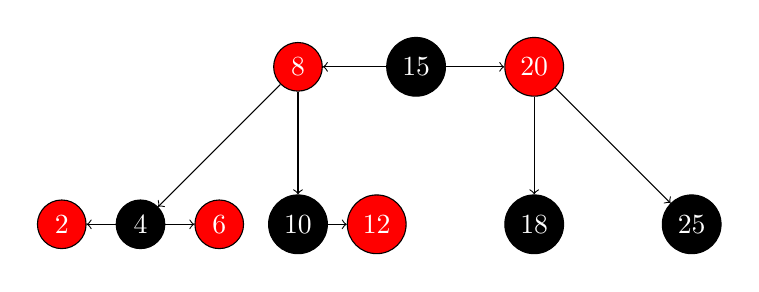
\begin{tikzpicture}
    \matrix[row sep=1cm, column sep=1cm] {
        \node[draw, fill=black, circle] (15) at (0, 0) {\textcolor{white}{15}};
        \node[draw, fill=red, circle] (8) at (-1.5, 0) {\textcolor{white}{8}};
        \node[draw, fill=red, circle] (20) at (1.5, 0) {\textcolor{white}{20}};
        \node[draw, fill=red, circle] (2) at (-4.5, -2) {\textcolor{white}{2}};
        \node[draw, fill=black, circle] (4) at (-3.5, -2) {\textcolor{white}{4}};
        \node[draw, fill=red, circle] (6) at (-2.5, -2) {\textcolor{white}{6}};
        \node[draw, fill=black, circle] (10) at (-1.5, -2) {\textcolor{white}{10}};
        \node[draw, fill=red, circle] (12) at (-0.5, -2) {\textcolor{white}{12}};
        \node[draw, fill=black, circle] (18) at (1.5, -2) {\textcolor{white}{18}};
        \node[draw, fill=black, circle] (25) at (3.5, -2) {\textcolor{white}{25}};

        \draw[->] (15) -- (8);
        \draw[->] (8) -- (4);
        \draw[->] (4) -- (2);
        \draw[->] (4) -- (6);
        \draw[->] (8) -- (10);
        \draw[->] (10) -- (12);
        \draw[->] (15) -- (20);
        \draw[->] (20) -- (25);
        \draw[->] (20) -- (18);
        \\
    };
\end{tikzpicture}
\end{document}
